\chapter{Resultados e discussão}\label{chp:resultados}

\section{Difusão de etinilestradiol nas matrizes poliméricas}

A \Figura{fig:difusao_adesivo} mostra a difusão de EE ao longo da camada polimérica do anel vaginal (posição em \textmu m) em diferentes dias, para $D_1 = 5,76 \times 10^{-13}$.  A concentração de EE permanece alta na maior parte da matriz, com uma diminuição acentuada nas bordas, refletindo as condições de contorno impostas e indicando uma maior resistência para a difusão.

Já na \Figura{fig:difusao_anel}, pode ser observada a difusão de EE ao longo da camada polimérica (posição em cm) em cada semana, para $D_2 = 7,92 \times 10^{-7}$. Nesse caso, a concentração de EE diminui gradualmente ao longo das semanas, indicando uma liberação contínua do fármaco.

\begin{figure}[!htb]
    \centering
        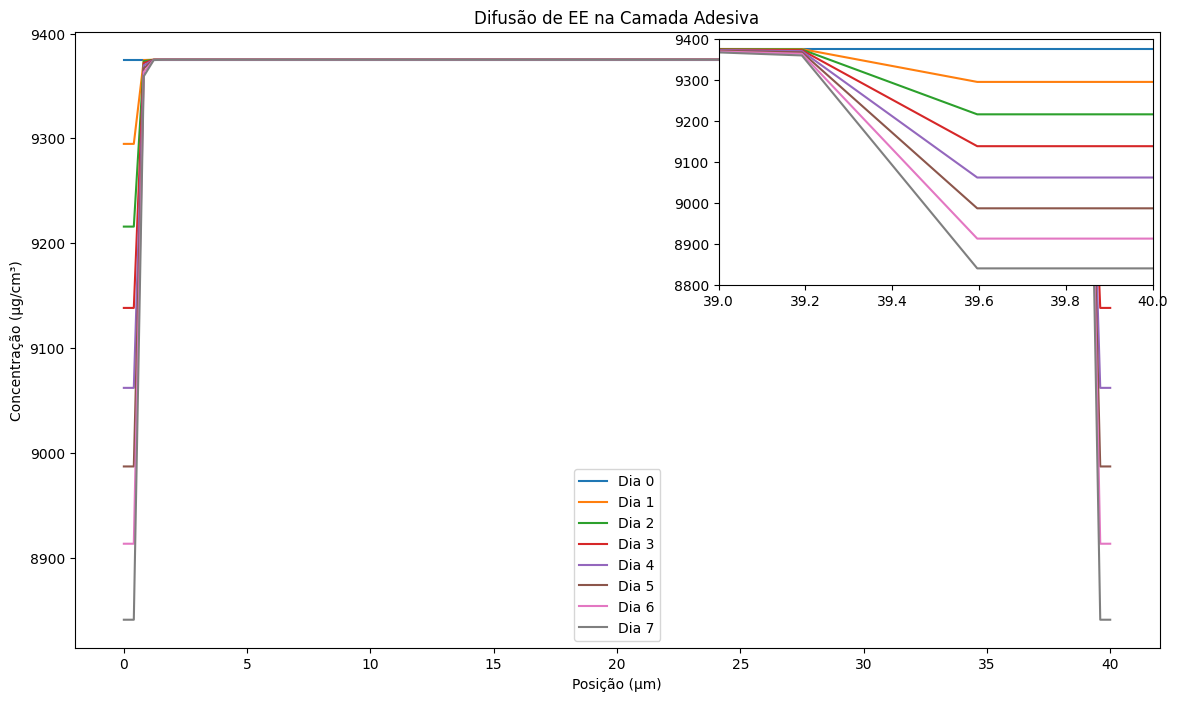
\includegraphics[width=1\textwidth]{figuras/difusao_adesivo.png}
        \caption[Difusão de etinilestradiol ao longo da camada adesiva]{Perfil obtido para a difusão de etinilestradiol ao longo da camada adesiva, para $D_1 = 5,76 \times 10^{-13}$. No canto superior direito, tem-se a região da extremidade ($0 < x < 1\mu m$) ampliada para melhor visualização da variação de concentração ao longo dos dias.}
    \label{fig:difusao_adesivo}
\end{figure}

\begin{figure}[!htb]
    \centering
        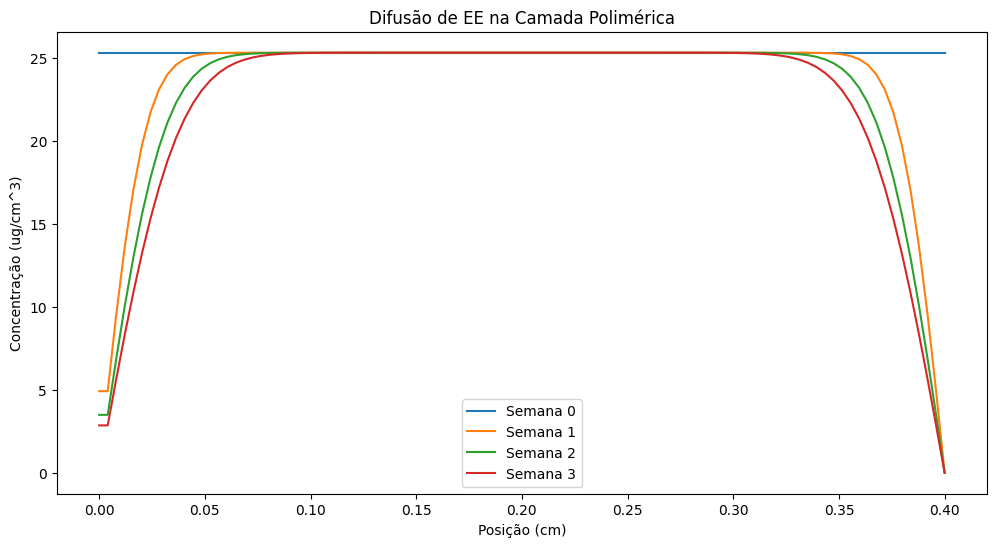
\includegraphics[width=1\textwidth]{figuras/difusao_anel.png}
        \caption[Difusão de etinilestradiol ao longo da camada polimérica do anel]{Perfil obtido para a difusão de etinilestradiol ao longo da camada polimérica do anel vaginal, para $D_2 = 7,92 \times 10^{-7}$.}
    \label{fig:difusao_anel}
\end{figure}

Ambos os perfis podem ser comparados com a \Figura{fig:Higuchi1961}, de Higuchi (1961), que esquematiza a difusão de um soluto de uma matriz polimérica para um fluido assumido como um sumidouro perfeito, fazendo com que a concentração de soluto nunca se acumule o suficiente para alterar a força motriz da difusão. Essa condição é válida para situações em que a concentração do soluto é muito maior do que a concentração de saturação, ou seja, a matriz está inicialmente saturada com soluto dissolvido. 

\begin{figure}[!htb]
    \centering
        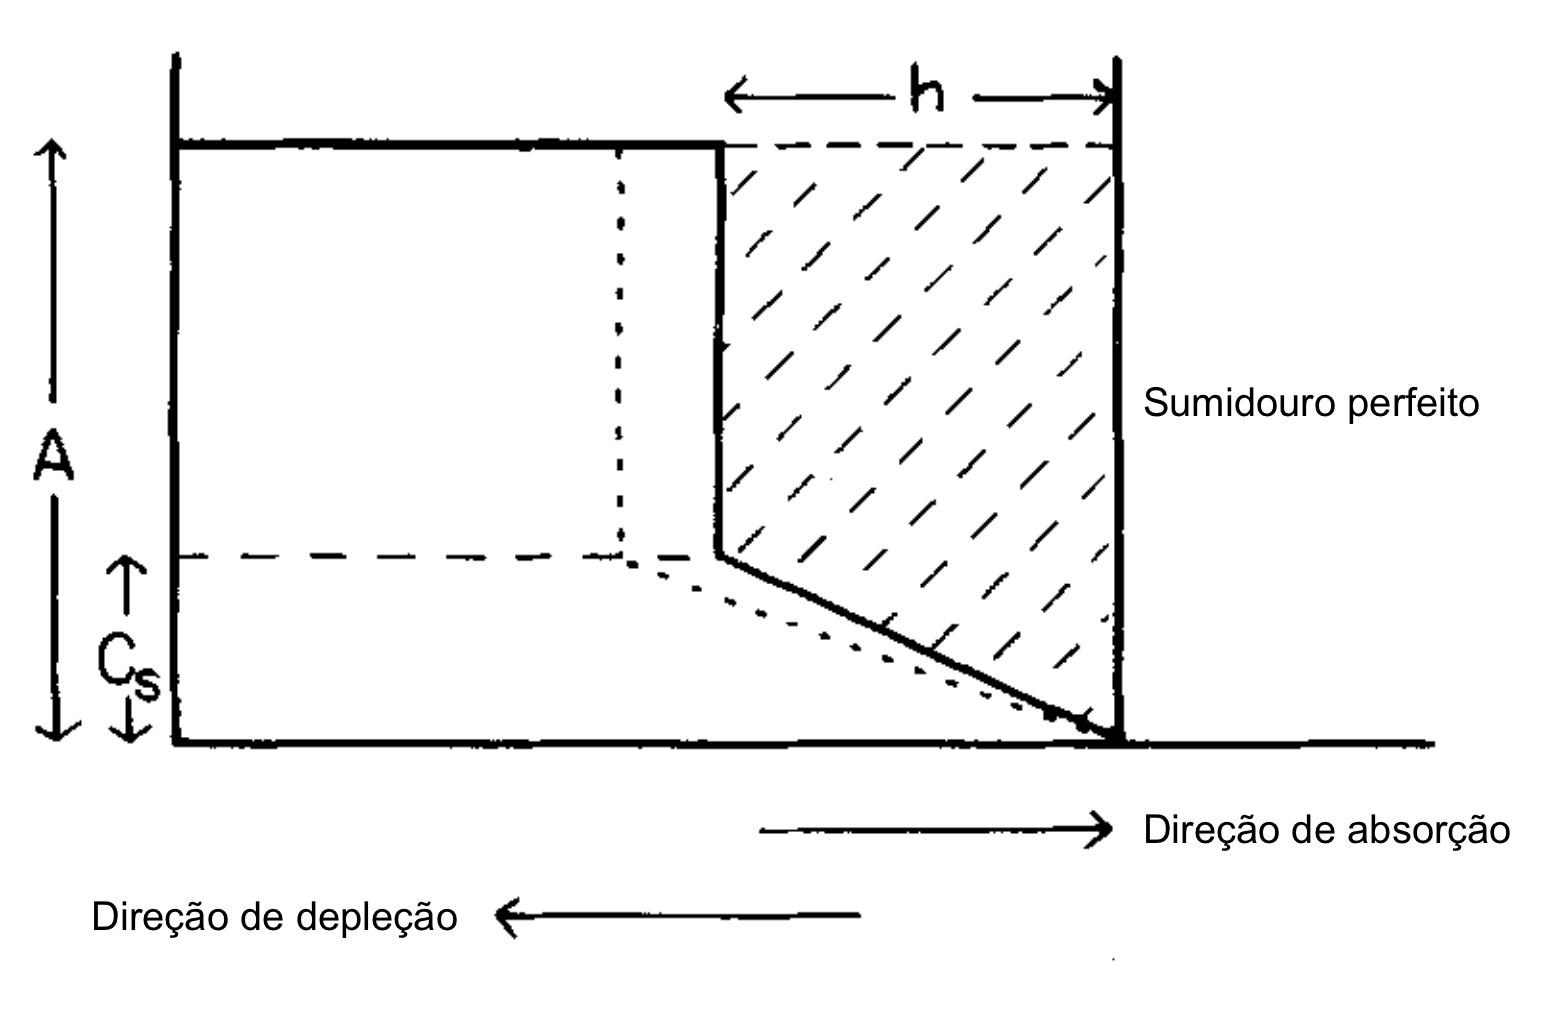
\includegraphics[width=0.6\textwidth]{figuras/Higuchi1961.png}
        \caption[Perfil de concentração teórica de uma matriz contendo fármaco em contato com um sumidouro perfeito]{Perfil de concentração teórica ao longo de uma matriz contendo fármaco em contato com um sumidouro perfeito (Higuchi, 1961).}
    \label{fig:Higuchi1961}
\end{figure}

Segundo Scheindlin (2004), em fármacos de liberação transdermal, um grande excesso de princípio ativo é colocado nos adesivos para manter o gradiente de concentração favorável à absorção. Assume-se aqui que esse seja o caso do etinilestradiol, extrapolando também para o anel vaginal. Sendo assim, pode ser observado que o perfil de difusão ao longo da camada polimérica do anel na região próxima da pele se assemelha à \Figura{fig:Higuchi1961}. Isso se deve à condição de contorno utilizada nessa borda, que assume a pele como um sumidouro perfeito devido a se tratar de uma mucosa. Na extremidade em contato com a solução, é possível perceber que a concentração não chega a zero, mas também não atinge o valor da concentração inicial. Isso é explicado pelo fato de ter sido estabelecida uma condição de fluxo zero em $x=0$, devido à consideração de que há uma quantidade finita de fármaco dentro do anel, e o fluxo ocorre em apenas uma direção.

Para o perfil de difusão ao longo da camada adesiva, é observado que apresenta, na extremidade $x = L$, um comportamento bem diferente da \Figura{fig:Higuchi1961}. Esse comportamento é esperado, considerando que o modelo foi desenvolvido considerando uma alta resistência nessa extremidade, criada pela pele. Essa condição é oposta à do sumidouro perfeito, portanto pode-se considerar que o modelo se adequa à realidade.

\section{Liberação de etinilestradiol ao longo do tempo}

\subsection{Liberação a partir do contraceptivo oral combinado}

A \Figura{fig:liberacao_coc} apresenta a concentração de etinilestradiol liberada a partir de uma pílula anticoncepcional no fluido gastrointestinal ao longo do tempo. É observado que a concentração de EE aumenta de forma contínua ao longo do tempo, atingindo um pico ao final do período de 24 horas. Ao se comparar com a referência da literatura para liberação de fármaco de primeira ordem, apresentada na \Figura{fig:primeira_ordem}, pode-se concluir que a curva obtida a partir do modelo apresenta o formato esperado, porém demora muito mais tempo para atingir os 80\% de liberação cumulativa do fármaco. Isso pode ser relacionado com os coeficientes $C_s$ e $k_d$ obtidos da literatura, ou com a própria natureza do COC de apresentar uma liberação controlada.

\begin{figure}[!htb]
    \centering
        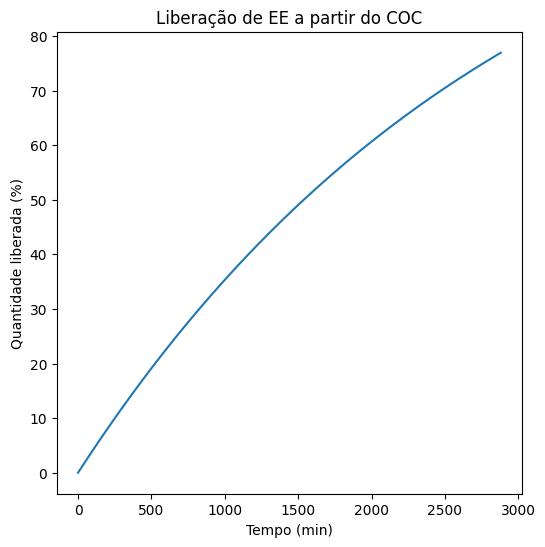
\includegraphics[width=0.46\textwidth]{figuras/liberacao_coc.png}
        \caption[Liberação cumulativa a partir do COC]{Quantidade de etinilestradiol (\%) liberada a partir do COC ao longo do tempo (min).}
    \label{fig:liberacao_coc}
\end{figure}

\begin{figure}[!htb]
    \centering
        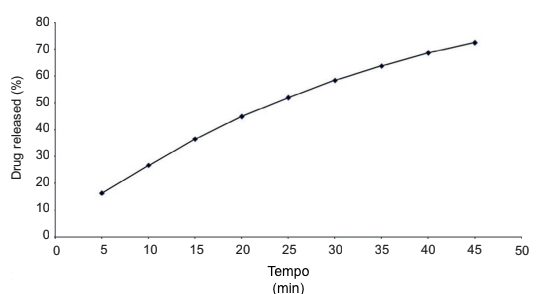
\includegraphics[width=0.6\textwidth]{figuras/primeira_ordem.png}
        \caption[Liberação de fármaco de primeira ordem]{Liberação de fármaco de primeira ordem: liberação cumulativa de fármaco (\%) versus tempo (min) (Bruschi, 2015).}
    \label{fig:primeira_ordem}
\end{figure}

\subsection{Taxa de liberação para cada matriz}

A fim de comparar as três diferentes matrizes estudadas entre si, foram plotadas as concentrações liberadas (\textmu g/mL) por tempo (dias) para cada uma delas, simulando a reposição no caso do COC e do adesivo, e abrangendo, assim, um período de 21 dias. O resultado é apresentado na \Figura{fig:liberacao_combinada}. Nela, podem ser observados picos regulares e decaimentos rápidos para a concentração liberada a partir do COC, uma liberação mais constante para o adesivo transdérmico e, por fim, uma liberação inicial rápida, seguida de uma estabilização em uma concentração mais baixa para o anel vaginal.

Esse gráfico pode ser comparado com a \Figura{fig:Heuvel}, obtida por Heuvel et. al (2005) a partir das concentrações plasmáticas das mulheres que participaram do estudo com cada um dos métodos contraceptivos. É perceptível que as concentrações obtidas na simulação foram muito mais altas do que as disponíveis na literatura, entretanto foi possível obter um perfil, no geral, muito similar para todas as matrizes estudadas.

\begin{figure}[!htb]
    \centering
        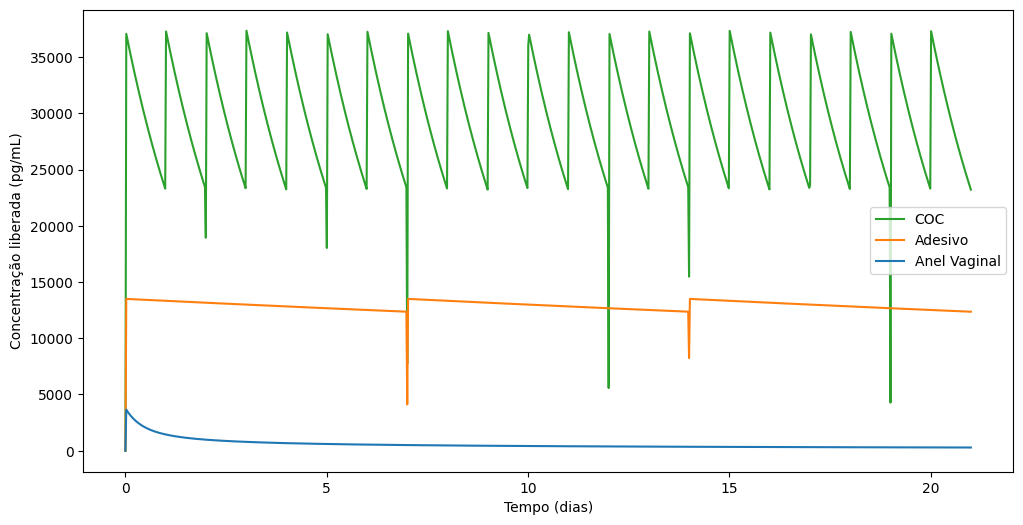
\includegraphics[width=1\textwidth]{figuras/liberacao_combinada.png}
        \caption[Liberação de etinilestradiol simulada ao longo do tempo]{Simulação da liberação de etinilestradiol (pg/mL) para o COC, adesivo e anel vaginal ao longo de 21 dias.}
    \label{fig:liberacao_combinada}
\end{figure}

\begin{figure}[!htb]
    \centering
        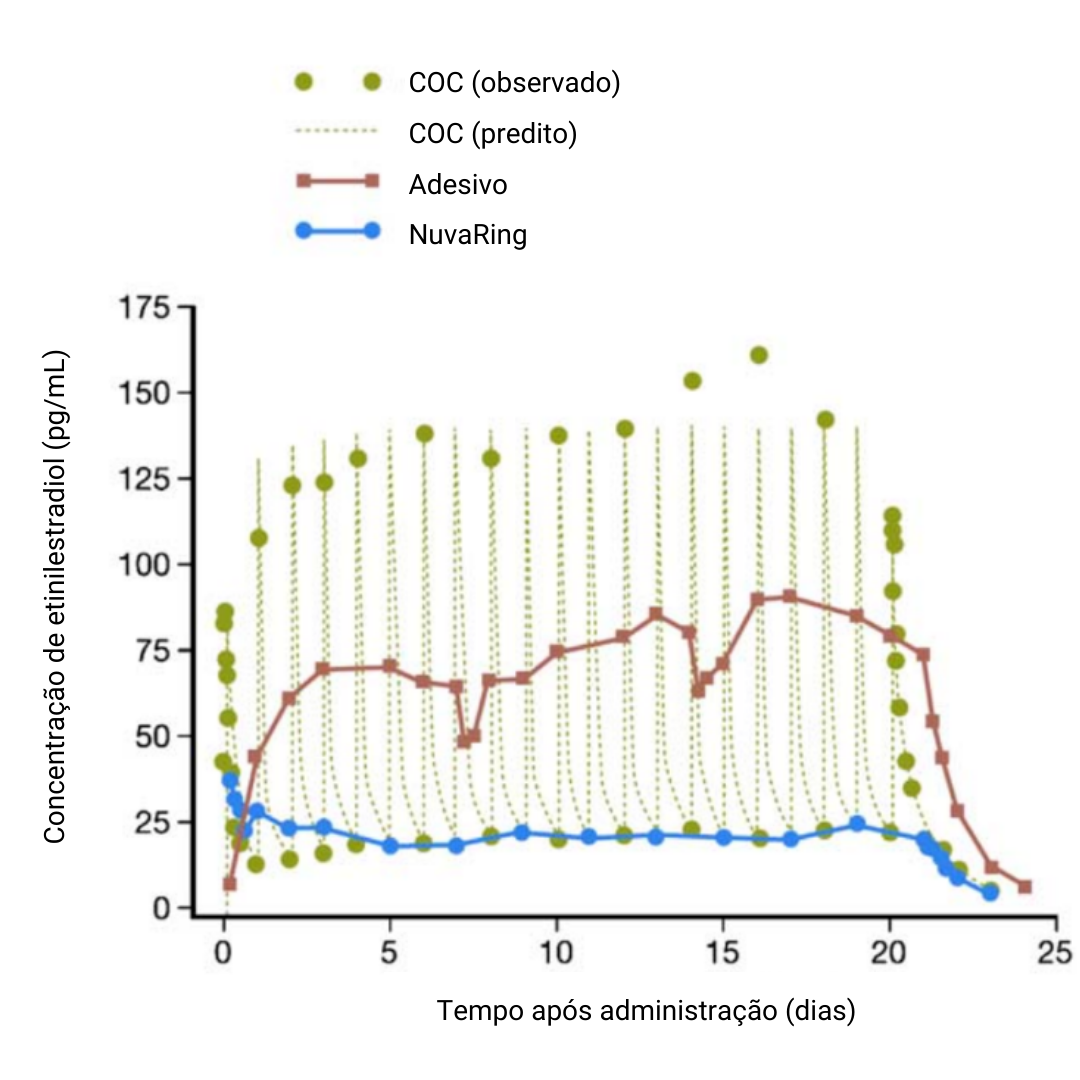
\includegraphics[width=0.68\textwidth]{figuras/Heuvel.png}
        \caption[Curvas experimentais de concentrações plasmáticas de EE]{Curvas obtidas a partir das concentrações plasmáticas de mulheres utilizando COC, adesivo e anel vaginal (Heuvel et. al, 2005)}
    \label{fig:Heuvel}
\end{figure}

A simulação realizada apresenta resultados coerentes com as afirmações da literatura de que a dosagem diária da pílula produz picos e vales na concentração de EE no sangue ao longo do tempo, enquanto o anel vaginal proporciona uma dosagem muito menor e mais estável (Heuvel et al. 2005). Além disso, observa-se que, de fato, a fim de compensar o metabolismo de primeira passagem, são liberadas concentrações mais elevadas do princípio ativo no COC do que nas demais matrizes (Kuhl, 2005). Corrobora-se também o fato de que o anel vaginal possui um efeito de liberação inicial rápida antes de atingir um estado estacionário na taxa de liberação, devido ao acúmulo de hormônios na superfície durante o armazenamento (Faundes, 2004).

A discrepância nos valores absolutos evidencia as limitações do modelo, advindas da desconsideração do metabolismo e eliminação do fármaco, fatores que provavelmente causam uma diminuição drástica nas concentrações plasmáticas. Dado que o objetivo principal desse trabalho diz respeito à modelagem da liberação de etinilestradiol, e não de sua concentração no sangue, essas limitações são aceitáveis dentro do escopo deste estudo. No entanto, para uma aplicação posterior, seria necessário integrar processos farmacocinéticos ao modelo, como metabolismo, distribuição, eliminação e absorção do fármaco. Além disso, ajustes nos parâmetros do modelo, como coeficientes de difusão e concentrações iniciais, com base em dados experimentais, poderiam melhorar a precisão das simulações e a aplicabilidade. 

\section{Análise de sensibilidade}

Os coeficientes de difusão nas matrizes poliméricas utilizados para os resultados apresentados foram selecionados com base nos valores das estimativas iniciais, mas multiplicados por fatores de conversão conforme o necessário, com o objetivo de obter resultados que permanecessem dentro da faixa esperada para a liberação do etinilestradiol nas matrizes analisadas. Essa abordagem permite uma análise preliminar da dinâmica de liberação, porém, sem uma precisão absoluta quanto aos valores dos coeficientes. Por isso, além da comparação com a literatura, foi realizada uma análise de sensibilidade com o intuito de demonstrar como variações nos coeficientes de difusão impactam cada uma das matrizes.

Para o adesivo transdérmico, o coeficiente de difusão que melhor se ajustou às condições físicas foi $D = 5,76 \times 10^{-13}$, isto é, 90000 vezes menor do que a estimativa original utilizada. Esse valor foi utilizado como base para a análise de sensibilidade realizada, comparando o perfil de difusão na extremidade em contato com a pele para $-50\% D$, $D$ e $+50\%D$. Os resultados estão dispostos na \Figura{fig:sensibilidade_adesivo}, onde pode ser observada uma maior diferença de concentração conforme se aumenta o valor de $D$. Assim, pode-se concluir que um valor maior de $D$ resulta em uma difusão mais rápida do 
fármaco, levando a uma diminuição mais rápida da concentração ao longo da espessura. Isso significa que, quanto menor o $D$, maior a resistência do meio à difusão, porém, uma variação pequena não produz resultados tão significativos. Esse fato pode explicar o motivo de ter sido necessário utilizar um valor tão mais baixo do que o inicial a fim de controlar melhor o perfil de liberação nessa matriz. É importante lembrar que não foi realizada uma simulação considerando a resistência da pele, então parte dessa resistência pode ter sido incorporada a esse modelo, levando a um $D$ mais baixo do que o da camada adesiva na realidade.

\begin{figure}[!htb]
    \centering
    \subfloat[$0,5D = 2,88 \times 10^{-13}$]{%
        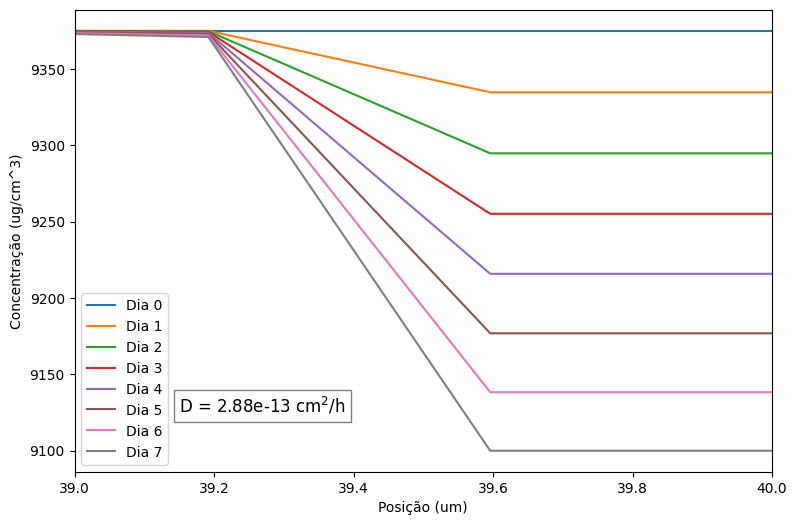
\includegraphics[width=0.65\textwidth]{figuras/sensibilidade_adesivo_05.png}%
        \label{fig:sensibilidade_adesivo_05}%
    }\\
    \subfloat[$D = 5,76 \times 10^{-13}$]{%
        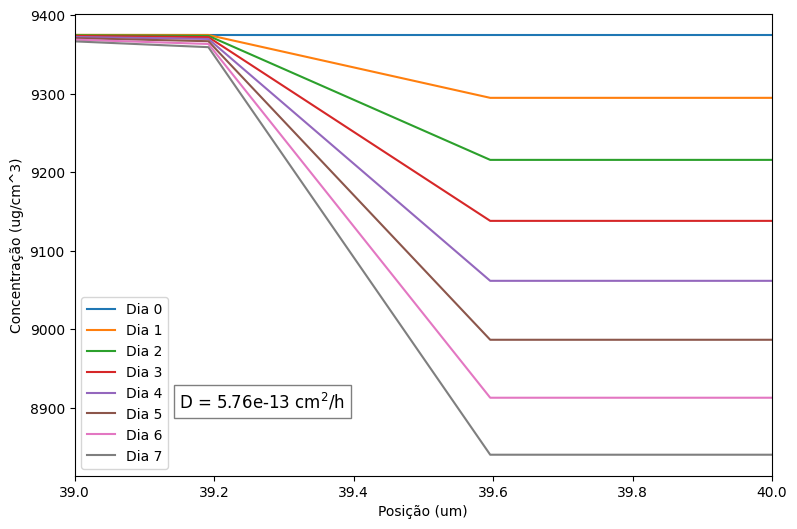
\includegraphics[width=0.65\textwidth]{figuras/sensibilidade_adesivo_1.png}%
        \label{fig:sensibilidade_adesivo_1}%
    }\\
    \subfloat[$1,5D = 8,64 \times 10^{-13}$]{%
        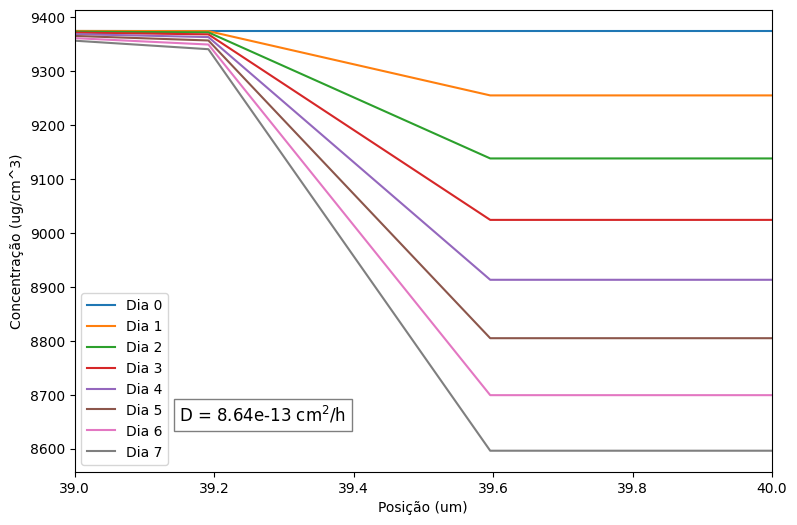
\includegraphics[width=0.65\textwidth]{figuras/sensibilidade_adesivo_50.png}%
        \label{fig:sensibilidade_adesivo_50}%
    }
    \caption[Análise de sensibilidade para o $D$ no adesivo transdérmico]{Análise de sensibilidade para o valor de $D$ no adesivo transdérmico, considerando \Subfigura{fig:sensibilidade_adesivo_05} -50\% $D$, \Subfigura{fig:sensibilidade_adesivo_1} $D$ e \Subfigura{fig:sensibilidade_adesivo_50} +50\% $D$}
    \label{fig:sensibilidade_adesivo}
\end{figure}

Para o anel vaginal, o coeficiente de difusão que melhor se ajustou às condições físicas foi $D = 7,92 \times 10^{-7}$, que é 5000 vezes menor do que o valor da estimativa inicial. Novamente, esse foi o valor foi utilizado como base para a análise de sensibilidade, comparando o perfil de difusão na extremidade em contato com a pele para $-50\% D$, $D$ e $+50\%D$. Os resultados estão dispostos na \Figura{fig:sensibilidade_anel}. Neles, pode ser novamente observada uma diminuição ligeiramente mais acentuada da concentração ao longo da posição quanto maior o valor de $D$, indicando menor resistência à difusão. O valor final bem maior do que o do adesivo, por si só, também corrobora o fato que se trata de um sistema com menor resistência, devido à aplicação ser em uma mucosa.

\begin{figure}[!htb]
    \centering
    \subfloat[$0,5D = 3,96 \times 10^{-7}$]{%
        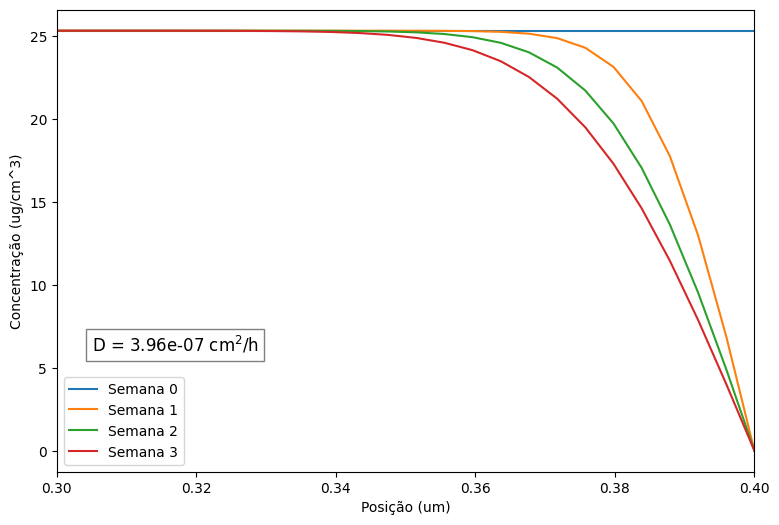
\includegraphics[width=0.62\textwidth]{figuras/sensibilidade_anel_05.png}%
        \label{fig:sensibilidade_anel_05}%
    }\\
    \subfloat[$D = 7,92 \times 10^{-7}$]{%
        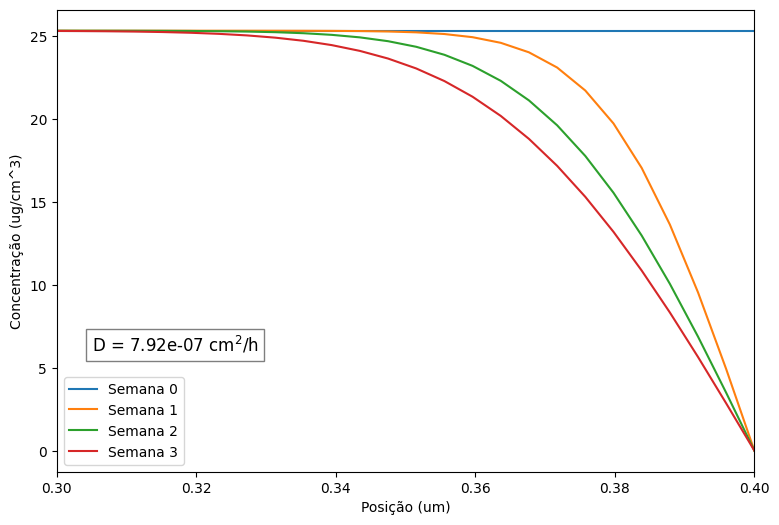
\includegraphics[width=0.62\textwidth]{figuras/sensibilidade_anel_1.png}%
        \label{fig:sensibilidade_anel_1}%
    }\\
    \subfloat[$1,5D = 1,19 \times 10^{-6}$]{%
        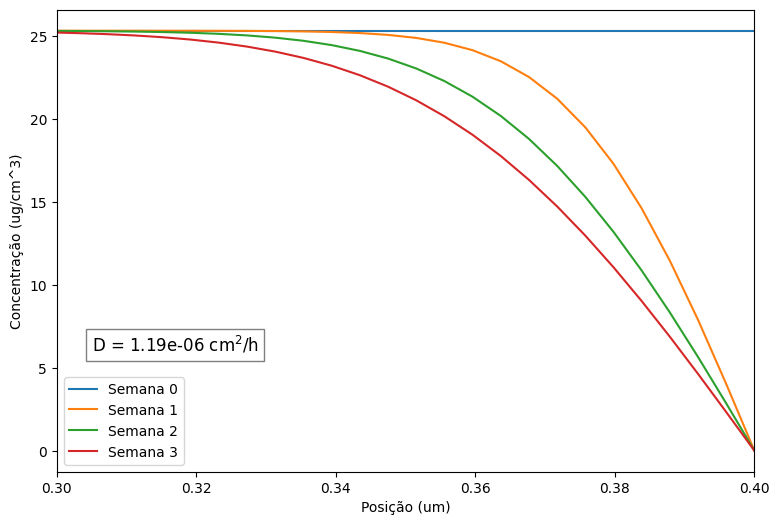
\includegraphics[width=0.62\textwidth]{figuras/sensibilidade_anel_50.png}%
        \label{fig:sensibilidade_anel_50}%
    }
    \caption[Análise de sensibilidade para o $D$ no anel vaginal]{Análise de sensibilidade para o valor de $D$ no anel vaginal, considerando \Subfigura{fig:sensibilidade_anel_05} -50\% $D$, \Subfigura{fig:sensibilidade_anel_1} $D$ e \Subfigura{fig:sensibilidade_anel_50} +50\% $D$}
    \label{fig:sensibilidade_anel}
\end{figure}

Por último, é importante ressaltar que já era esperado que os coeficientes de difusão para essas duas matrizes fossem menores do que os obtidos na literatura, afinal, ambos os valores eram para o $17\beta$-estradiol, que é uma molécula de raio menor, e portanto apresenta menos resistência à difusão. 